% !TeX encoding = UTF-8
% !TeX root = ../main.tex

%% ------------------------------------------------------------------------
%% Copyright (C) 2021 SJTUG
%% 
%% SJTUBeamer Example Document by SJTUG
%% 
%% SJTUBeamer Example Document is licensed under a
%% Creative Commons Attribution-NonCommercial-ShareAlike 4.0 International License.
%% 
%% You should have received a copy of the license along with this
%% work. If not, see <http://creativecommons.org/licenses/by-nc-sa/4.0/>.
%% -----------------------------------------------------------------------

\section{Introduction}

\subsection{Background}

%\begin{frame}{Motivation}
%  Reasons behind my research paper choice:
%  \begin{itemize}
%    \item My research line is mainly targeted to blockchain technology
%    \item This specific research paper has been developed by my PhD co-supervisors (good chance to learn about their researching style)
%    \item My PhD thesis could use some of the model simulation techniques (stochastic processes) used in this research paper experimentation
%    \item And of course, it is related to a emerging subfield that could greatly contribute to the development of the Internet of Things (IoT)
%  \end{itemize}
%\end{frame}

\begin{frame}[fragile]{Background}

  Blockchain technology $\rightarrow$ theoretical potential:
  \begin{itemize}
		\item Data integrity
		\item Decentralizing trust
		\item Reducing costs
  \end{itemize}
	
  Useful practical application? $\rightarrow$ \alert{e-government} (software administration processes)
    
   \begin{exampleblock}{From generic case to more specific}
    	\textbf{studenty mobility management} $\subset$ supply chain management
  \end{exampleblock}

\end{frame}

%\subsection{Crowdsensing}
%
%\begin{frame}{Crowdsensing: definition}
%  \begin{itemize}
%  \item \textbf{Crowdsensing:} emerging paradigm of data aggregation\cite{paper1}, having a key role in data-driven applications. Specially used for getting large ammounts of IoT sensing data, by using the individual intelligent sensing devices.
%  \item \textbf{Benefit:} improved data collection efficiency and reduced costs effectively\cite{paper2}
%  \end{itemize}
%  \begin{figure}[h]
%        \centering
%        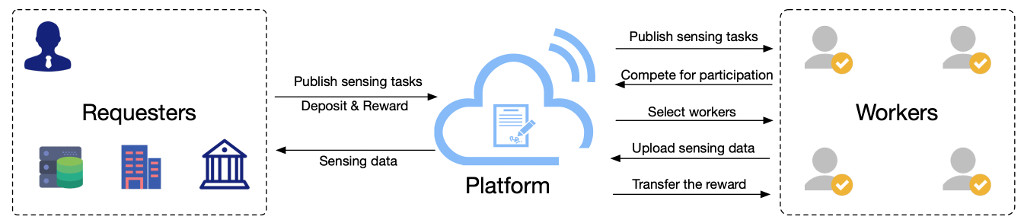
\includegraphics[width=.8\textwidth]{201909-wei-figure1.jpg}
%      \end{figure}
%\end{frame}
%
%\begin{frame}{Crowdsensing: issues}
%  		\begin{enumerate}
%   			\item Managed and maintained \alert{centralized platforms} suffer from the single point of failure
%   				\begin{itemize}
%   					\item \textbf{Proposal: } decentralized architecture (blockchain technology) that lacks a single point of failure, and enhances privacy with asymmetric encryption and digital signature technology
%   				\end{itemize}
%    		\item Encouraging workers by offering appropiate \alert{incentive mechanisms} (monetary usually) \rightarrow  \underline{auction theory} guarantees benefits for both requesters and workers\cite{paper15} but only provide short-term incentives
%    			\begin{itemize}
%   					\item \textbf{Proposal:} hybrid incentive mechanism, adopting \underline{mechanism design theory}, considering three factors:
%   					\begin{itemize}
%   					\item Monetary reward
%   					\item Reputation evaluation
%   					\item Data quality
%   					\end{itemize}
%   				\end{itemize}
%  		\end{enumerate}
%\end{frame}
